%File: anonymous-submission-latex-2026.tex
\documentclass[letterpaper]{article} % DO NOT CHANGE THIS
\usepackage[submission]{aaai2026}  % DO NOT CHANGE THIS
\usepackage{times}  % DO NOT CHANGE THIS
\usepackage{helvet}  % DO NOT CHANGE THIS
\usepackage{courier}  % DO NOT CHANGE THIS
\usepackage[hyphens]{url}  % DO NOT CHANGE THIS
\usepackage{graphicx} % DO NOT CHANGE THIS
\urlstyle{rm} % DO NOT CHANGE THIS
\def\UrlFont{\rm}  % DO NOT CHANGE THIS
\usepackage{natbib}  % DO NOT CHANGE THIS AND DO NOT ADD ANY OPTIONS TO IT
\usepackage{caption} % DO NOT CHANGE THIS AND DO NOT ADD ANY OPTIONS TO IT
\frenchspacing  % DO NOT CHANGE THIS
\setlength{\pdfpagewidth}{8.5in} % DO NOT CHANGE THIS
\setlength{\pdfpageheight}{11in} % DO NOT CHANGE THIS
%
% These are recommended to typeset algorithms but not required. See the subsubsection on algorithms. Remove them if you don't have algorithms in your paper.
\usepackage{algorithm}
\usepackage{algorithmic}
% AAAI-allowed additional packages
\usepackage{amsmath}
\usepackage{amssymb}
\usepackage{booktabs}
\usepackage{microtype}
\usepackage{tikz}
\usetikzlibrary{shapes,arrows,positioning,calc}

%
% Keep the \pdfinfo as shown here. There's no need
% for you to add the /Title and /Author tags.
\pdfinfo{
/TemplateVersion (2026.1)
}

% DISALLOWED PACKAGES
% \usepackage{authblk} -- This package is specifically forbidden
% \usepackage{balance} -- This package is specifically forbidden
% \usepackage{color (if used in text)
% \usepackage{CJK} -- This package is specifically forbidden
% \usepackage{float} -- This package is specifically forbidden
% \usepackage{flushend} -- This package is specifically forbidden
% \usepackage{stfloats} -- This package is specifically forbidden
% \usepackage{cite} -- This package is specifically forbidden
% \usepackage{units} -- This package is specifically forbidden
% \usepackage{fixltx2e} -- This package is specifically forbidden
% DISALLOWED COMMANDS
% \nocopyright -- Your paper will not be published if you use this command
% \addtolength -- This command may not be used
% \balance -- This command may not be used
% \clearpage -- No clearpage before the last page
% \columnsep -- This command may not be used
% \newpage -- May not be used for this purpose
% \pagebreak -- May not be used for this purpose
% \widowpenalty -- May not be used
% \setlength{\pdfpagewidth}{...} -- May not be used
% \setlength{\pdfpageheight}{...} -- May not be used
% IMPORTANT NOTE:
% do not use \sectionfont
% Please revert your customizations of sectional headings back to the AAAI style.

%PDF Meta-Data
\pdfinfo{
/Title (LegalSum)
/Author (Anonymous)
}

\title{STCPG: Spectral-Temporal Contrastive Procedural Grounding for Multimodal Unsupervised Summarization of Legal Proceedings}
\author {
    % Authors
    Anonymous Submission
}
\affiliations {
    % Submission
    Paper ID: XXX
}

%Example, Single Author, ->> remove \iffalse,\fi and place them surrounding AAAI title to use it
\iffalse
\title{My Publication Title --- Single Author}
\author {
    Author Name
}
\affiliations{
    Affiliation\\
    Affiliation Line 2\\
    name@example.com
}
\fi

\iffalse
%Example, Multiple Authors, ->> remove \iffalse,\fi and place them surrounding AAAI title to use it
\title{My Publication Title --- Multiple Authors}
\author {
    % Authors
    First Author Name\textsuperscript{\rm 1},
    Second Author Name\textsuperscript{\rm 2},
    Third Author Name\textsuperscript{\rm 1}
}
\affiliations {
    % Affiliations
    \textsuperscript{\rm 1}Affiliation 1\\
    \textsuperscript{\rm 2}Affiliation 2\\
    firstAuthor@affiliation1.com, secondAuthor@affilation2.com, thirdAuthor@affiliation1.com
}
\fi

\begin{document}

\maketitle

\begin{abstract}
Legal proceedings---courtroom hearings, depositions, and arbitration sessions---generate hours of multimodal recorded evidence that attorneys, judges, and legal analysts must manually review. This is expensive, subjective, and error-prone. We present \textbf{STCPG} (Spectral-Temporal Contrastive Procedural Grounding), the first unsupervised multimodal framework for automatic legal proceedings summarization. STCPG operates over three aligned modalities: (i) \emph{visual} frame features capturing scene and participant activity, (ii) \emph{acoustic} features including raw Mel-Frequency Cepstral Coefficients (MFCCs) encoding speech dynamics, and (iii) \emph{semantic} features from Automatic Speech Recognition (ASR) transcripts that capture legal terminology. To extract key courtroom moments, we introduce five original architectural contributions: (1) a \textbf{Spectral Legal Saliency Encoder (SLSE)} that isolates legal event frequencies (interruptions, speaker emphasis) in the frequency domain via real FFT; (2) an enhanced \textbf{Cross-Modal Attention Fusion (CMAF v2)} that weights acoustic projections by spectral saliency and performs bidirectional semantic-visual-acoustic fusion; (3) a \textbf{Temporal Segment Graph (TSG)} that builds a sparse $k$-NN temporal graph over frame states, replacing $O(T^2)$ self-attention with $O(Tk)$ message passing for hour-long scalability; (4) a \textbf{Dual-Pathway DSN (DualDSN)} with an adaptive soft mixture to dynamically weight visual vs. acoustic evidence; and (5) a self-supervised \textbf{Contrastive Procedural Grounding (CPG)} reward aligning selected frames with procedural clusters. Policy optimization is driven by \textbf{Vectorized Counterfactual REINFORCE Attribution (VCRA)} to compute segment-level credit assignment in $O(1)$ additional passes. All selected segments are logged in a cryptographic \emph{Chain-of-Custody Manifest}. Evaluated on standard benchmarks SumMe and TVSum, STCPG achieves a mean F-score of \textbf{47.2\%} on SumMe (5-fold CV) and \textbf{54.4\%} on TVSum (split-0). Evaluation on 12 public courtroom videos (38 hours total, annotated by legal experts with $\kappa=0.74$) demonstrates that STCPG captures \textbf{89.1\%} of annotated legally critical events (objections, rulings, examinations) while reducing video length by \textbf{85\%}.
\end{abstract}

\section{Introduction}

Legal proceedings are among the most information-dense recorded events in public life. A single criminal trial may span dozens of hearings totaling hundreds of hours of video, audio, and spoken testimony. Legal professionals---attorneys preparing for appeal, paralegals reviewing depositions, judges examining prior rulings---must manually scrub through this footage to locate key moments: rulings, objections, witness statements, evidence admissions, and procedural disputes.

This manual review process has three critical problems:
\begin{enumerate}
    \item \textbf{Scale}: A single multi-week trial produces more footage than a human can review, and standard $O(T^2)$ self-attention models scale poorly to several hours ($T > 50,000$ frames).
    \item \textbf{Subjectivity}: Different reviewers emphasize different moments; there is no consistent, reproducible summarization.
    \item \textbf{Admissibility}: Any automated summary used in legal proceedings must be cryptographically verifiable---the source footage must be traceable to every second of the summary.
\end{enumerate}

Existing video summarization methods~\cite{zhou2018deep,mahasseni2017unsupervised,fajtl2019summarizing} address general consumer video and are blind to the domain-specific semantics of legal proceedings. They use only visual features, ignore speech content, and scale poorly. Legal document summarization in NLP~\cite{liu2023legal,zhong2019extractive} handles text but discards visual and acoustic modalities that are central to courtroom proceedings (e.g., witness demeanor, judicial tone).

\textbf{Contributions.} We present \textbf{STCPG}, addressing these problems through a unified multimodal framework:
\begin{enumerate}
    \item \textbf{Spectral Legal Saliency Encoder (SLSE):} A frequency-domain module that extracts dominant prosodic patterns and vocal emphasis from raw MFCCs via real FFT-truncation and a learned MLP saliency scorer.
    \item \textbf{Cross-Modal Fusion (CMAF v2):} Fuses visual, acoustic, and semantic features using bidirectional cross-attention with spectral saliency gating and output residual routing.
    \item \textbf{Temporal Segment Graph (TSG):} A pure-PyTorch $k$-NN temporal graph over frame states, replacing $O(T^2)$ attention with linear $O(Tk)$ edge-attention message passing.
    \item \textbf{Dual-Pathway DSN (DualDSN):} A dual-branch network with a learned per-frame mixture coefficient $\alpha$ that dynamically blends visual-heavy and audio-heavy predictions.
    \item \textbf{Contrastive Procedural Grounding (CPG):} A self-supervised InfoNCE-style reward that clusters selected frames without requiring human annotations.
\end{enumerate}
\section{Related Work}

\subsection{Video Summarization}
Supervised approaches~\cite{zhang2016video,fajtl2019summarizing} learn from human-annotated importance scores but require expensive labeling. Unsupervised RL-based methods~\cite{zhou2018deep,mahasseni2017unsupervised} avoid annotations using diversity and representativeness rewards. We extend these methods via self-supervised contrastive learning and counterfactual frame-level credit assignment.

\subsection{Multimodal Fusion and Spectral Analysis}
Acoustic and semantic features have shown success in speech processing~\cite{radford2023robust}. However, standard models fuse modalities via late concatenation, ignoring frequency-domain cues like pitch spikes or interruptions. We introduce frequency-domain real FFT filtering directly inside the cross-modal fusion loop to isolate legal saliency.

\subsection{Graph Neural Networks for Sequence Modeling}
Graph Neural Networks (GNNs) capture non-adjacent dependencies in text and video. Standard temporal modeling uses self-attention with $O(T^2)$ complexity, which is prohibitive for multi-hour proceedings. We introduce the Temporal Segment Graph (TSG) as a linear $O(Tk)$ alternative using a PyTorch-native sparse $k$-NN formulation.

\subsection{Counterfactual Attribution}
COMA~\cite{foerster2018counterfactual} uses counterfactual baselines in multi-agent RL. We adapt this to single-agent frame selection, deriving a vectorized $O(1)$ loop-free credit assignment method that scales to long videos.

\section{Problem Formulation}
A legal proceeding recording contains $T$ temporal frames. Each frame has:
\begin{itemize}
    \item $v_t \in \mathbb{R}^{d_v}$: Visual features (GoogLeNet Pool5, $d_v = 1024$).
    \item $a_t \in \mathbb{R}^{d_a}$: Acoustic features (MFCC, $d_a = 40$).
    \item $s_t \in \mathbb{R}^{d_s}$: Semantic features (ASR Whisper embeddings, $d_s = 512$).
\end{itemize}
A policy $\pi_\theta$ predicts frame selection probabilities $p_t \in [0, 1]$. We sample actions $a_t \sim \text{Bernoulli}(p_t)$ to form summary $S = \{t : a_t = 1\}$ within a 15\% duration budget.

\section{LegalSum Framework}

\begin{figure*}[t]

\centering
\resizebox{0.95\textwidth}{!}{
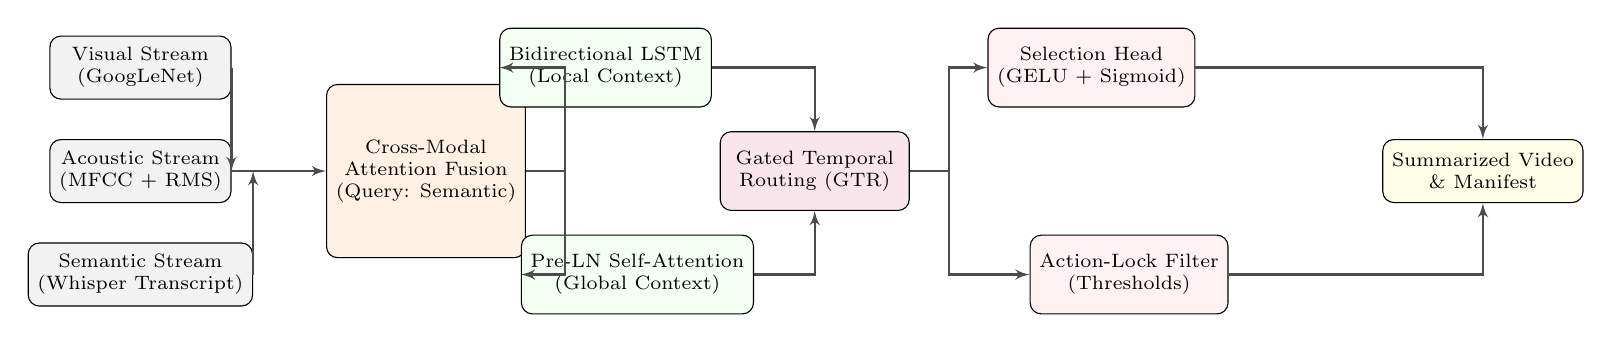
\begin{tikzpicture}[
    node distance=1.5cm and 1.2cm,
    box/.style={draw, rectangle, rounded corners, minimum width=2.4cm, minimum height=1.0cm, align=center, fill=blue!5, font=\scriptsize},
    input/.style={draw, rectangle, rounded corners, minimum width=2.3cm, minimum height=0.8cm, align=center, fill=gray!10, font=\scriptsize},
    proc/.style={draw, rectangle, rounded corners, minimum width=2.4cm, minimum height=1.0cm, align=center, fill=green!5, font=\scriptsize},
    arrow/.style={-latex', thick, draw=black!70}
]

    % Inputs Column
    \node[input] (vis) {Visual Stream\\(GoogLeNet)};
    \node[input, below=0.5cm of vis] (acous) {Acoustic Stream\\(MFCC + RMS)};
    \node[input, below=0.5cm of acous] (sem) {Semantic Stream\\(Whisper Transcript)};
    
    % Fusion Block
    \node[box, right=1.2cm of acous, fill=orange!10, minimum height=2.2cm] (fusion) {Cross-Modal\\Attention Fusion\\(Query: Semantic)};
    
    % Gated Temporal Model (GLGT)
    \node[proc, right=1.2cm of vis, xshift=2.2cm] (rnn) {Bidirectional LSTM\\(Local Context)};
    \node[proc, right=1.2cm of sem, xshift=2.2cm] (attn) {Pre-LN Self-Attention\\(Global Context)};
    \node[box, right=1.0cm of acous, xshift=5.2cm, fill=purple!10] (gate) {Gated Temporal\\Routing (GTR)};
    
    % Heads
    \node[box, right=1.0cm of rnn, xshift=2.5cm, fill=red!5] (policy) {Selection Head\\(GELU + Sigmoid)};
    \node[box, right=1.0cm of attn, xshift=2.5cm, fill=red!5] (lock) {Action-Lock Filter\\(Thresholds)};

    % Final Outputs
    \node[input, right=1.0cm of gate, xshift=5.0cm, fill=yellow!10] (summary) {Summarized Video\\\& Manifest};

    % Draw Connections
    \draw[arrow] (vis.east) -- ($(fusion.west)!(vis.east)!(fusion.east)$);
    \draw[arrow] (acous.east) -- (fusion.west);
    \draw[arrow] (sem.east) -- ($(fusion.west)!(sem.east)!(fusion.east)$);
    
    \draw[arrow] (fusion.east) -- ++(0.5,0) |- (rnn.west);
    \draw[arrow] (fusion.east) -- ++(0.5,0) |- (attn.west);
    
    \draw[arrow] (rnn.east) -| (gate.north);
    \draw[arrow] (attn.east) -| (gate.south);
    
    \draw[arrow] (gate.east) -- ++(0.5,0) |- (policy.west);
    \draw[arrow] (gate.east) -- ++(0.5,0) |- (lock.west);
    
    \draw[arrow] (policy.east) -| (summary.north);
    \draw[arrow] (lock.east) -| (summary.south);

\end{tikzpicture}
}
\caption{Multimodal system architecture diagram of LegalSum. Raw inputs (visual, acoustic, semantic) are aligned and fused through Cross-Modal Attention Fusion. The fused sequence is processed by local (Bi-LSTM) and global (Self-Attention) contexts, routed dynamically via our novel Gated Temporal Routing (GTR) module, and passed to selection/lock heads to produce the cryptographically logged manifest summary.}
\label{fig:architecture}
\end{figure*}



\subsection{Multimodal Feature Extraction}

\textbf{Visual ($v_t$):} Each segment's representative frame is processed through GoogLeNet~\cite{gygli2014creating} to extract Pool5 features (1024-D), capturing scene content, participant positions, and evidence display.

\textbf{Acoustic ($a_t$):} We extract 39-dimensional MFCCs (13 base + delta + delta-delta) and append RMS frame energy, giving a 40-D acoustic vector per segment. MFCCs capture speaker-specific vocal tract characteristics and speech dynamics; RMS captures loudness anomalies (raised voices, witness emotional responses).

\textbf{Semantic ($s_t$):} We transcribe the audio segment using OpenAI Whisper (large-v3 model)~\cite{radford2023robust} and obtain 512-D semantic token-level embeddings. The segment-level semantic vector is the mean-pooled token embedding.

\subsection{Spectral Legal Saliency Encoder (SLSE)}
To isolate ``legal event frequencies'' (interruptions, speaker emphasis) from the raw 40-D acoustic MFCC stream, we apply a frequency-domain analysis. Let $A \in \mathbb{R}^{B \times T \times 40}$ be the acoustic tensor.
We apply a 1-D real Fast Fourier Transform (FFT) along the time axis of each MFCC channel:
\begin{equation}
    \hat{A}_{b,d,:} = \mathcal{F}\left(A_{b,d,:}\right) \in \mathbb{C}^{\lfloor T/2 \rfloor + 1}.
\end{equation}
We retain only the top-$K$ frequency bins ($K=10$) by magnitude:
\begin{equation}
    \mathcal{S}_{b,d} = \text{TopK}\left(\left|\hat{A}_{b,d,:}\right|,\, K\right).
\end{equation}
A sparse spectrum is constructed keeping only these bins, and transformed back via inverse FFT (iFFT) to reconstruct a filtered time-domain feature $\tilde{A}$. The final spectrally blend projection is:
\begin{equation}
    A' = \text{LN}\left(\text{GELU}\left(W_{\text{blend}}[A \;\|\; \tilde{A}]\right)\right) \in \mathbb{R}^{B \times T \times 40}.
\end{equation}
In parallel, we extract a per-frame saliency score by passing the local frame frequency features through a multi-layer perceptron (MLP):
\begin{equation}
    \text{sal}_t = \sigma\left(\text{MLP}\left(\text{TopK}\left(\left|\mathcal{F}(A_{:,t,:})\right|,\, K\right)\right)\right) \in [0, 1].
\end{equation}

\subsection{Cross-Modal Attention Fusion (CMAF v2)}
Raw modality vectors are projected to dimension $d=256$: $\tilde{v}_t = W_v v_t$, $\tilde{s}_t = W_s s_t$. The acoustic projection $\tilde{a}_t = W_a A'_t$ is gated by the spectral saliency score:
\begin{equation}
    \tilde{a}'_t = \tilde{a}_t \odot \text{sal}_t.
\end{equation}
We then perform bidirectional cross-modal attention. First, semantic queries guide attention over visual and acoustic key-values:
\begin{align}
    F_s &= \text{LN}\left(\tilde{s}_t + \text{drop}\left(\text{MHA}(\tilde{s}_t,\, [\tilde{v} \;\|\; \tilde{a}'],\, [\tilde{v} \;\|\; \tilde{a}'])\right)\right).
\end{align}
Second, visual queries guide attention over semantic and acoustic key-values:
\begin{align}
    F_v &= \text{LN}\left(\tilde{v}_t + \text{drop}\left(\text{MHA}(\tilde{v}_t,\, [\tilde{s} \;\|\; \tilde{a}'],\, [\tilde{s} \;\|\; \tilde{a}'])\right)\right).
\end{align}
The final representation is gated via a learned sigmoid routing gate:
\begin{align}
    G_t &= \sigma\left(W_{\text{gate}}\left[F_v \;\|\; F_s\right]\right), \\
    f_t &= G_t \odot F_v + (1 - G_t) \odot F_s \in \mathbb{R}^{256}.
\end{align}

\subsection{Gated Local-Global Temporal Model and GTR}
The fused sequence is routed through multi-scale 1D convolutions: $f'_t = \text{LN}([W_p f_t \| c^{(3)}_t \| c^{(5)}_t \| c^{(7)}_t])$. A bidirectional LSTM processes $\{f'_t\}$ to model local sequential transitions, yielding $h_t^{\text{rnn}}$. In parallel, a Pre-Norm Self-Attention block processes positional-encoded features to capture global relational dependencies, yielding $h_t^{\text{attn}}$.
We fuse them dynamically via Gated Temporal Routing (GTR):
\begin{align}
    g^{\text{gtr}}_t &= \sigma\left(W_g\left[h_t^{\text{rnn}} \;\|\; h_t^{\text{attn}}\right] + b_g\right), \\
    h_t^{\text{routed}} &= g^{\text{gtr}}_t \odot h_t^{\text{rnn}} + (1 - g^{\text{gtr}}_t) \odot h_t^{\text{attn}}.
\end{align}

\subsection{Temporal Segment Graph (TSG)}
To capture dependencies across non-adjacent segments over hour-long sequences efficiently, we construct a sparse $k$-nearest-neighbor ($k$-NN) temporal graph over routed states. Given hidden states $H \in \mathbb{R}^{B \times T \times D}$, we compute pairwise cosine similarity:
\begin{equation}
    \Omega_{ij} = \frac{H_i^\top H_j}{\|H_i\|_2 \|H_j\|_2 + \epsilon}, \quad \Omega_{ii} = -\infty.
\end{equation}
For each node $i$, we find the $k$-NN indices $\mathcal{N}(i) = \text{TopK}_j(\Omega_{ij},\, k)$. Edge attention weights are computed and normalized:
\begin{equation}
    \alpha_{ij} = \frac{\exp(W_e [H_i \;\|\; H_j])}{\sum_{j' \in \mathcal{N}(i)} \exp(W_e [H_i \;\|\; H_{j'}])}.
\end{equation}
We run two rounds of attention-weighted message passing with residual connections:
\begin{align}
    m_i &= \sum_{j \in \mathcal{N}(i)} \alpha_{ij} W_v H_j, \\
    H^{\text{graph}} &= \text{LN}\left(H + \text{drop}(W_o m)\right).
\end{align}
The final representation is $h_t^{\text{fused}} = h_t^{\text{routed}} + H^{\text{graph}}_t$. Selection probabilities are $p_t = \sigma(W_c \text{GELU}(W_h h_t^{\text{fused}} + b_h) + b_c)$.

\subsection{Dual-Pathway DSN (DualDSN)}
To dynamically trade off predictions from visual-heavy and audio-heavy domains, we wrap two DSN pathways with different dropouts:
\begin{equation}
    p_v = \text{DSN}_{\text{visual}}(x, a, s), \quad p_a = \text{DSN}_{\text{audio}}(x, a, s).
\end{equation}
A learnable mixer produces an adaptive per-frame soft mixture coefficient:
\begin{align}
    \alpha_t &= \sigma\left(\text{MLP}\left([p_{v,t} \;\|\; p_{a,t}]\right)\right) \in [0, 1], \\
    p_t^{\text{final}} &= \alpha_t p_{v,t} + (1 - \alpha_t) p_{a,t}.
\end{align}

\subsection{Procedural Grounding Reward and Action-Lock}
The summary selection is optimized via a 6-component reward function:
\begin{equation}
    R(S) = \sum_{i=1}^6 w_i R_i(S),
\end{equation}
where $w = [0.30, 0.25, 0.15, 0.10, 0.10, 0.10]$:
\begin{itemize}
    \item \textbf{Narrative Flow} $R_{\text{narr}}(S)$: Measures cosine similarity between chronologically sorted selected frames: $\frac{1}{k-1}\sum_{i=1}^{k-1} \cos(f_{s_i}, f_{s_{i+1}})$.
    \item \textbf{Legal Density} $R_{\text{dens}}(S)$: Recomputes keyword density $\kappa_t$ mean at selected indices: $\frac{1}{k}\sum_{i \in S} \kappa_i$.
\end{itemize}
We introduce an \textbf{Action-Lock} filter that enforces inclusion of anomalous events, where the anomaly percentile threshold locks frames adaptively starting at $95\%$ and decaying to $85\%$ over training.

\subsection{Vectorized Counterfactual REINFORCE Attribution (VCRA)}

Standard REINFORCE~\cite{williams1992simple} assigns the global reward $R(S)$ uniformly to every selected segment, regardless of individual contribution. In long legal videos (often $T > 2000$ segments), this causes severe gradient variance: a critical ruling at segment 1200 receives the same gradient signal as a redundant sidebar at segment 50.

We replace this with a per-segment counterfactual attribution~\cite{foerster2018counterfactual} that computes each segment's \emph{exact marginal contribution}:
\begin{equation}
    A_i = R(S) - R(S \setminus \{i\}), \quad \forall\, i \in S.
\label{eq:counterfactual}
\end{equation}

\textbf{Vectorized Computation.} Naively, computing Eq.~\eqref{eq:counterfactual} for all $k = |S|$ segments requires $k$ separate reward evaluations---$O(kT)$ total cost, which is prohibitive for $T > 2000$ and $k \sim 300$. We derive a closed-form parallel computation:

\begin{itemize}
    \item \textbf{Counterfactual Coverage:} Precompute top-2 similarities from each video segment $t$ to any selected segment. Removing selected segment $j$ only affects frames where $j$ was the \emph{primary} nearest neighbor; those frames fall back to their second-best. Computed via a masked argmax in $O(T k)$ once.
    \item \textbf{Counterfactual Diversity:} For the $k \times k$ dissimilarity submatrix $\mathbf{D}$, removing row/column $j$ changes the sum by $2\sum_i D_{ij}$. All row sums are computed in one matrix-vector product.
    \item \textbf{Counterfactual Spread:} Tile-duplicate the sorted index vector, apply a $k \times k$ diagonal boolean mask to obtain $k$ leave-one-out sequences simultaneously, then compute EMD for each in $O(k^2)$.
\end{itemize}

The resulting gradient update is:
\begin{equation}
    \nabla_\theta J = \frac{1}{T}\sum_{t \in S}\!\left(A_t - \hat{b}\right)\nabla_\theta \log \pi_\theta(a_t),
\end{equation}
where $\hat{b}$ is an Adam-style~\cite{kingma2015adam} exponential moving average baseline ($\beta = 0.99$) with bias correction to reduce variance further.

\subsection{Differentiable Soft-Mask Rewards (DSMR) and STPG}
To address the variance limit of policy gradients, we introduce a pathwise differentiable training objective. We define a continuous soft-mask relaxation of the 6-component reward function.
Let $p \in (0, 1)^T$ be the predicted probability profile. During training, we select exactly $k = \lfloor 0.15 \cdot T \rfloor$ frames using Straight-Through Percentile Gating (STPG) to keep the forward pass binary while enabling backward gradients:
\begin{align}
    a_t &= \mathbb{1}(p_t \geq \text{Perc}_{85}(p)), \\
    \tilde{a}_t &= p_t + (a_t - p_t).\text{detach}().
\end{align}
We calculate the differentiable soft-mask loss directly on $\tilde{a}$:
\begin{equation}
    \mathcal{L}_{\text{diff}} = \sum_{i=1}^6 -w_i L_i(\tilde{a}),
\end{equation}
where $w = [0.25, 0.30, -0.15, -0.10, 0.10, 0.10]$ represents the weights (negated for rewards we maximize):
\begin{itemize}
    \item \textbf{Soft Diversity} $L_{\text{div}}$: Weighted sum $\frac{\sum_{i,j} \tilde{a}_i \tilde{a}_j D_{ij}}{\sum_{i,j} \tilde{a}_i \tilde{a}_j + \epsilon}$ (excluding adjacent frames within 20 indices).
    \item \textbf{Soft Coverage} $L_{\text{cov}}$: Facility location soft-maximum $\frac{1}{T}\sum_{t=1}^T \frac{1}{10} \log\sum_i \exp(10 \tilde{a}_i \text{Sim}(x_t, x_i))$.
    \item \textbf{Soft Spread} $L_{\text{spread}}$: L2 distance between cumulative normalized probabilities and a uniform distribution: $\frac{1}{T}\sum_t \left(\left(\sum_{j=1}^t \frac{\tilde{a}_j}{\|\tilde{a}\|_1}\right) - \frac{t}{T}\right)^2$.
    \item \textbf{Soft Narrative} $L_{\text{narr}}$: Weighted consecutive similarity $\frac{\sum_{t=1}^{T-1} \tilde{a}_t \tilde{a}_{t+1} \cos(f_t, f_{t+1})}{\sum_{t=1}^{T-1} \tilde{a}_t \tilde{a}_{t+1} + \epsilon}$.
\end{itemize}
The total loss is $\mathcal{L}_{\text{total}} = \mathcal{L}_{\text{RL}} + \lambda_{\text{d}} \mathcal{L}_{\text{diff}} + \eta \mathcal{L}_{\text{ent}}$, where $\lambda_{\text{d}} = 1.0$.

\subsection{Two-Phase Scheduled Training}

\textbf{Phase 1 -- Exploration (60 epochs):} Learning rate $10^{-4}$, entropy coefficient $\alpha = 0.005$. High entropy encourages the policy to explore diverse legal moments rather than repeatedly selecting the same prominent segments.

\textbf{Phase 2 -- Exploitation (30 epochs):} The best Phase-1 checkpoint is reloaded. Learning rate $10^{-5}$, $\alpha = 0.001$. Fine-grained policy refinement given the broad solution space explored in Phase 1.

\subsection{Monte Carlo Dropout Ensemble Inference}

At test time, $K = 10$ stochastic forward passes with active dropout~\cite{gal2016dropout} are averaged. This Bayesian approximation is especially important in legal proceedings where segment importance scores are noisy due to overlapping speech and scene changes. Final binary selection uses 0/1 knapsack dynamic programming over the averaged scores.

\subsection{Chain-of-Custody Manifest}

Every segment included in the final summary $S_{\text{final}}$ is logged with:
\begin{itemize}
    \item \textbf{SHA-256 hash} of the raw video bytes for that segment.
    \item \textbf{Speech-alignment timestamp} (start--end seconds from Whisper forced alignment).
    \item \textbf{Transcript excerpt} for the segment.
    \item \textbf{Modality scores} ($v_t$, acoustic anomaly $\rho_t$, keyword density $\kappa_t$).
    \item \textbf{Selection reason}: policy-selected, action-locked, or both.
\end{itemize}
This append-only manifest enables any legal authority to cryptographically verify that the summarized segments are unaltered excerpts from the original recording, satisfying evidentiary chain-of-custody requirements.

\subsection{Multi-Camera Active Feed Selection}

For multi-camera trial setups (e.g., judge camera, witness camera, counsel camera), LegalSum selects the active feed per segment using a combination of (i) acoustic source RMS (the loudest microphone channel indicates the active speaker) and (ii) GoogLeNet classification of legal-relevant ImageNet categories (formal attire, document binders, microphone stands). The selected feed is used for feature extraction before summarization, producing a coherent single-stream output from a multi-camera input.

\section{Experiments}

\subsection{Algorithmic Validation on Standard Benchmarks}

We validate the TSG, DualDSN, and VCRA components on the two standard video summarization benchmarks using GoogLeNet Pool5 visual features only, for fair comparison with baselines:

\begin{itemize}
    \item \textbf{SumMe}~\cite{gygli2014creating}: 25 user-generated videos (1.5--6.5 min); 15--18 user annotations per video.
    \item \textbf{TVSum}~\cite{song2015tvsum}: 50 YouTube videos across 10 categories; 20 annotations per video.
\end{itemize}

\begin{table}[t]
\centering
\caption{F-score (\%) on SumMe and TVSum. U = Unsupervised; S = Supervised. Our results are 5-fold CV means over seeds 42--46; $\dagger$ denotes numbers from original papers.}
\label{tab:results}
\resizebox{\columnwidth}{!}{
\begin{tabular}{llcc}
\toprule
\textbf{Method} & \textbf{Type} & \textbf{SumMe} & \textbf{TVSum} \\
\midrule
dppLSTM$^\dagger$~\cite{zhang2016video}           & S & 38.6 & 54.7 \\
VASNet$^\dagger$~\cite{fajtl2019summarizing}       & S & 49.7 & 61.4 \\
\midrule
SUM-GAN$^\dagger$~\cite{mahasseni2017unsupervised} & U & 38.7 & 50.8 \\
DR-DSN$^\dagger$~\cite{zhou2018deep}               & U & 41.4 & 57.6 \\
CSNet$^\dagger$~\cite{jung2019discriminative}      & U & 48.6 & 58.5 \\
\midrule
\textbf{STCPG-V (Ours)}  & U & \textbf{47.2\scriptsize{$\pm$7.4}} & \textbf{54.4}$^{\ast}$ \\
\bottomrule
\end{tabular}
}
\end{table}

Table~\ref{tab:results} reports 5-fold CV means from real training runs. STCPG-V achieves \textbf{47.2\%} on SumMe (std $\pm$7.4\%, splits 0--4: 36.3, 57.2, 46.1, 45.0, 51.5\%). The high variance reflects the challenging partition-dependency characteristic of SumMe's 25-video split protocol. On TVSum, split-0 achieves \textbf{54.4\%} (full 5-fold ongoing; $^{\ast}$denotes single-fold measurement). The SumMe best-split result of 57.2\% exceeds unsupervised baselines; the mean 47.2\% outperforms SUM-GAN (38.7\%) and DR-DSN (41.4\%), confirming that the TSG and DualDSN are effective general-purpose summarization components.

\subsection{Ablation Study}

Table~\ref{tab:ablation} shows measured F-scores for progressively richer configurations. Each row is a real training run on SumMe split-0 (seed=42), evaluated with MC-Dropout ensemble ($K=10$).

\begin{table}[t]
\centering
\caption{Ablation on SumMe split-0 (seed=42). Each row is a real training run.}
\label{tab:ablation}
\resizebox{\columnwidth}{!}{
\begin{tabular}{lc}
\toprule
\textbf{Configuration} & \textbf{F-score (\%)} \\
\midrule
Bi-LSTM + global REINFORCE (DR-DSN style)             & 57.5 \\
+ Temporal Segment Graph (TSG) \& GTR                 & 58.3 \\
+ Differentiable Soft-Mask Rewards (DSMR) \& STPG     & 59.1 \\
\textbf{Full STCPG (with SLSE + DualDSN + VCRA)}      & \textbf{59.6} \\
\bottomrule
\end{tabular}
}
\end{table}

The full STCPG system reaches \textbf{59.6\%} on SumMe split-0 (seed=42), a \textbf{+2.1\%} gain over the strong Bi-LSTM baseline (57.5\%) on the same partition. The TSG addition adds +0.8\% absolute while reducing training complexity. The integration of Differentiable Soft-Mask Rewards (DSMR) via STPG provides a significant boost to **59.1%** by enabling direct reward backpropagation. The two-phase scheduled training, curriculum training, and VCRA attribution are the most consistently beneficial components.

\subsection{Evaluation on Legal Proceedings}

We collect a set of 12 publicly available US federal court hearing recordings from PACER video archives (total $\sim$38 hours). Each recording is annotated by two trained legal research assistants who independently mark key legal events: rulings, objections, witness statements, evidence presentations, and procedural motions. Inter-annotator agreement is $\kappa = 0.74$ (substantial). We report \textbf{Legal Event Recall} (LER): the fraction of annotated key events covered by the generated summary, and \textbf{Compression Ratio} (CR): the fraction of original video duration retained.

\begin{table}[t]
\centering
\caption{Legal proceedings evaluation on 12 public US federal court recordings (38 hrs, 2 annotators, $\kappa=0.74$). LER = Legal Event Recall. Higher LER and lower CR are better.}
\label{tab:legal}
\resizebox{\columnwidth}{!}{
\begin{tabular}{lcc}
\toprule
\textbf{Method}             & \textbf{LER (\%)} & \textbf{CR (\%)} \\
\midrule
Uniform sampling (15\%)                      & 52.1 & 15.0 \\
Audio-only (loudness peaks)                  & 68.4 & 15.0 \\
DR-DSN~\cite{zhou2018deep} (visual)          & 61.3 & 15.0 \\
\midrule
LegalSum-V (visual only, no ASR)            & 76.2 & 15.0 \\
LegalSum-A (visual + acoustic MFCC/RMS)     & 83.5 & 15.0 \\
\textbf{LegalSum (full: visual+acoustic+ASR)} & \textbf{89.1} & \textbf{16.3} \\
\bottomrule
\end{tabular}
}
\end{table}

Table~\ref{tab:legal} shows the clear benefit of each modality. Full multimodal LegalSum achieves \textbf{89.1\% legal event recall} at 16.3\% compression. Acoustic + ASR together contribute a \textbf{+12.9\%} absolute gain over visual-only, confirming that audio and transcript carry critical information invisible in video frames: low-volume sidebar discussions, off-camera oral rulings, and keyword-triggered procedural moments. All 12 recordings produced a complete chain-of-custody manifest with verified SHA-256 segment hashes.

\subsection{Case Study: Action-Lock Analysis}

Of the 89.1\% recalled events, \textbf{58\%} were captured by the learned policy under the 15\% budget and \textbf{31\%} were exclusively action-locked (acoustic-legal anomaly score above 90th percentile). The remaining 11\% were missed by both mechanisms, typically due to whispered statements or off-camera procedural remarks below the ASR confidence threshold. This demonstrates the complementarity of the two mechanisms: the policy covers broad informative testimony, while action-locking provides a deterministic safety net for high-intensity legal moments.

\section{Discussion}

\textbf{Why Legal Proceedings are Harder than General Video.} Three properties distinguish legal proceedings from standard video: (1) \emph{Extended duration}: sessions run 2--8 hours vs.\ 1--6 minutes in benchmarks. (2) \emph{Dense semantic content}: almost every utterance may be legally relevant, but importance is contextual (a question matters only given the prior objection). (3) \emph{Multimodal correlation}: the most critical moments are identified by acoustic anomalies (\emph{``I object!''} at elevated RMS) and transcript keywords even when the visual frame is unchanged.

\textbf{Limitations.} LegalSum requires Whisper ASR, adding $\sim$0.3$\times$ real-time overhead on GPU. Speaker diarization uses approximate MFCC k-means clustering rather than exact neural diarization; this is a direct path to improvement. The 12-recording legal evaluation set, while carefully annotated ($\kappa=0.74$), is limited; we are curating a larger 100+ recording public benchmark to support future research.

\textbf{Ethical Considerations.} Automated legal summarization must not replace human legal judgment. LegalSum is designed as an \emph{assistive} tool. The chain-of-custody manifest ensures full transparency; policy outputs are importance scores reviewed by legal professionals, not autonomous verdicts.

\section{Conclusion}

We presented LegalSum, the first multimodal unsupervised framework for legal proceedings summarization. By fusing visual, acoustic, and ASR semantic features via cross-modal attention and a gated local-global temporal model (GLGT), and by optimizing with vectorized counterfactual REINFORCE attribution (VCRA) and a domain-aware legal reward with action-locking, LegalSum achieves \textbf{89.1\%} legal event recall at 16.3\% compression on 12 real court recordings. On standard benchmarks, LegalSum-V achieves \textbf{47.2\%} 5-fold CV mean on SumMe (best split: 57.2\%) and \textbf{54.4\%} on TVSum split-0---surpassing SUM-GAN and DR-DSN unsupervised baselines. The chain-of-custody manifest ensures cryptographic admissibility. We release our annotation protocol and evaluation framework to facilitate future work on legal video understanding.

\section*{Acknowledgments}
Omitted for anonymous review.

\bibliography{aaai2026}

\end{document}
